Now, how about irrational numbers? We can construct \(\sqrt{2}\) by constructing a isosceles triangle and taking the hypotenuse. What else?

Let \(F\) be the set of constructible real numbers.

\thm. Any \(\alpha \in F\) can be represented using combinations of \(+\), \(-\), \(\times\), \(\div\) and \(\sqrt{\vphantom{l}}\).

\pf Idea. We have a ruler and a compass, so we can use the equation of lines and circles. So we can \textit{only} get a combination of the above operations. Thus, if we can construct radicals, the theorem is trivial.

\begin{center}

    \usetikzlibrary {decorations.pathmorphing, decorations.pathreplacing, decorations.shapes}
    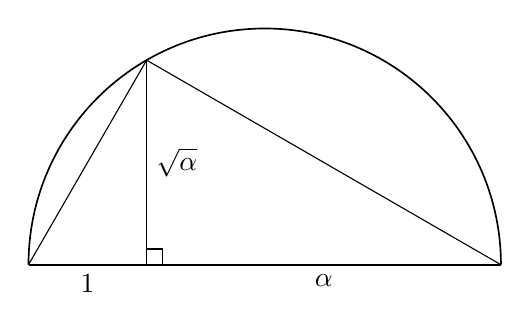
\begin{tikzpicture}
        \coordinate (A) at (-3, 0);
        \coordinate (B) at (3, 0);
        \coordinate (P) at (-1.5, 2.598);
        \coordinate (H) at (-1.5, 0);
        \draw[semithick] (A) arc(180:0:3) (B);
        \draw[semithick] (A) -- (B);
        \draw (P) -- (H) node[midway, right] {\(\sqrt{\alpha}\)};
        \draw (A) -- (P);
        \draw (B) -- (P);
        \draw (A) -- (H) node[midway, below] {\(1\)};
        \draw (B) -- (H) node[midway, below] {\(\alpha\)};
        \draw (H) rectangle (-1.3, 0.2);
    \end{tikzpicture}
\end{center}

\vspace*{-10pt}

\qed

Since we can use radicals, the degree of extension would be at most \(2\).

\cor. Let \(r\) be an irrational constructible number. Then there exists \(r_1, r_2, \dots, r_m = r \in \R\) such that
\[
    [\Q(r_1, \dots, r_l) : \Q(r_1, \dots, r_{l+1})] = 2
\]
for \(l = 1, 2, \dots, m - 1\). In particular, \([\Q(r) : \Q] = 2^n\) for some \(n \in \Z_{\geq 0}\).

\pf Each \(r_i\) occurs when we use radicals, so the existence of \(r_i\) is immediate, and radicals extend the field with degree \(2\), so the result follows. \qed

\section*{The Impossibility of Certain Constructions}

\thm. Doubling a cube is impossible. i.e, \(\sqrt[3]{2}\) is not constructible.

\pf Suppose that \(\sqrt[3]{2} \in F\). But \([\Q(\sqrt[3]{2}) : \Q] = 3\), which is not a power of \(2\). \qed

\thm. Squaring a circle is impossible. i.e, \(\sqrt{\pi}\) is not constructible.

\pf \(\pi\) is transcendental over \(\Q\), and so is \(\sqrt{\pi}\). \qed

\thm. Trisecting an arbitrary angle is impossible.

\pf Suppose we have an angle of \(60^\circ\). If constructing \(20^\circ\) is possible, then we can construct \(\cos 20^\circ\). Now we show that \(\cos 20^\circ\) is not constructible. From the identity \(\cos 3\theta = 4\cos^3 \theta - 3\cos\theta\), set \(\theta = 20^\circ\), and let \(\alpha = \cos \theta\). Then we have \(8\alpha^3 - 6\alpha - 1 = 0\), which is irreducible. Since \(\alpha\) is a zero, \([\Q(\alpha) : \Q] = 3\), which is a contradiction. \qed

\rmk Regular \(n\)-gon (\(n \geq 3\)) is constructible \(\iff\) the angle \(\frac{2\pi}{n}\) is constructible \(\iff\) \(\cos \frac{2\pi}{n}\) is constructible.

\pagebreak

\topic{Finite Fields}

Our goal is to determine the structure of all \textit{finite fields}, fields with finite order.

\thm. Let \(F\) be a finite field with \(\abs{F} = q\). If \(E\) is a finite extension of \(F\) with \([E : F] = n\), then \(\abs{E} = q^n\).

\pf \(E\) is an \(n\)-dimensional \(F\)-vector space. Trivial. \qed

\cor. Let \(E\) be a finite field with \(\ch E = p\). Then \(\abs{E} = p^n\) for some \(n \in \N\).\footnote{Note that \(p\) has to be prime.}

\pf Let \(1\) be the multiplicative identity of \(E\). Then \(\{1, 2 \cdot 1, \dots, p \cdot 1\} \simeq \Z_p \leq E\). Therefore \(E\) is a finite extension of a finite field \(\Z_p\), so we have \(\abs{E} = p^n\) for some \(n \in \N\). \qed

\thm. Let \(E \subset \bar{\Z_p}\) be a field with \(\ch E = p\) and \(\abs{E} = p^n\). Then
\begin{center}
    \(E \simeq \left\{ \text{zeros of } x^{p^n} - x \in \Z_p[x] \text{ in } \bar{\Z_p} \right\}\).
\end{center}

\pf Since \(E\) is a field, \(E\cross\) is a group and \(\abs{E\cross} = p^n - 1\). Then for \(a \in E\cross\), \(a^{\abs{E\cross}} = 1\). Thus \(a^{p^n - 1} - 1 = 0\), and \(a^{p^n} - a = 0\). Thus every element in \(E\) is a zer of \(x^{p^n} - x\). Since this polynomial can have at most \(p^n\) zeros, we are done. \qed

The zeros of the polynomial \(x^{p^n} - x \in \Z_p[x]\) describes \(E\).

\defn. \note{Root of Unity}
\begin{enumerate}
    \item \(\zeta\) is a \textbf{\(n\)-th root of unity} if \(\zeta^n = 1\).
    \item \(\zeta\) is a \textbf{primitive \(n\)-th root of unity} if \(\zeta^n = 1\) and \(\zeta^i \neq 1\) for \(1 \leq i < n\).
\end{enumerate}

\cor. If \(F\) is a finite field and \(E\) is a finite extension of \(F\), then \(E\) is a simple extension.

\pf \(E\cross\) is a cyclic group, so suppose that \(\alpha \in E\cross\) is a generator. Then \(E = F(\alpha)\) by definition of simple extensions. \qed

Suppose \(\Z_p \leq E = \Z_p(\alpha) \leq K = E(\beta)\), where \(\alpha\) is algebraic over \(\Z_p\) and \(\beta\) is algebraic over \(E\). Then these are finite extensions, so \(K\) is a simple extension of \(F\). i.e, \(K = F(\gamma)\) for some \(\gamma\). The extension depends on which element you choose.

\thm. For any prime \(p\) and \(n \in \N\), there exists a field \(E\) of order \(p^n\).

\pagebreak
